%\documentclass[10pt,landscape,twocolumn]{article}
\documentclass[10pt]{article}

%%% Langage et accents
	\usepackage[french]{babel} % Langue française
	\usepackage[T1]{fontenc}
	\usepackage[utf8]{inputenc}
	\usepackage{gentium}

%%% Packages
	\usepackage{fullpage,xcolor,graphicx}
	\usepackage{url}
	\usepackage{upgreek}
	\usepackage{lettrine}
	\usepackage{array}
	\usepackage[hidelinks]{hyperref}

%%% Couleur principale
	\definecolor{main}{HTML}{7E9AB7}%4A7FB7
	
%%% Géométrie
	%\usepackage[a4paper,margin=2cm,top=1.6cm]{geometry}
	\usepackage[a4paper,bottom=2.5cm]{geometry}
	\setlength{\columnsep}{15mm}

%%% Format des différents titres
	\usepackage{titlesec}
	\titleformat{\section}{\normalfont\LARGE\nobreak}{\thesection}{1em}{}
	\titleformat{\subsection}{\color{main!90!black}\normalfont\Large\nobreak}{\thesubsection}{1em}{}
	\titleformat{\subsubsection}{\color{main}\normalfont\nobreak}{\thesubsubsection}{1em}{}

%%% Cadres colorés
	\usepackage[many]{tcolorbox}
	\tcbset{skin=enhanced,boxrule=0.3pt,arc=2pt,lifted shadow={0.5mm}{-0.5mm}{1mm}{0.1mm}{black},enlarge top by=1mm,enlarge bottom by=1mm,colback=main!10!white,colframe=main}
	% Attention, les ombres nécéssitent la version 2014 de TeXLive !

%%% Commandes personalisées
	\newcommand{\gr}[1]{{\color{main}{#1}}}
	\newcommand{\cadre}[1]{\begin{tcolorbox}#1\end{tcolorbox}}


\title{\huge{Écrivez de vrais documents}}
\author{\emph{Une introduction au logiciel LaTeX}}

\begin{document}

% Page de titre
\maketitle
\vspace{30mm}
\begin{center}

\includegraphics[width=40mm]{figures/remington.pdf}
\vspace{10mm}


\includegraphics[width=14mm]{figures/cc}
\end{center}
\thispagestyle{empty}
\clearpage

% Table des matières
%\tableofcontents
%\clearpage

\section*{Introduction}

\lettrine[lines=3]{S}{i} vous êtes habitués à utiliser Word depuis l'école primaire, vous n'avez peut-être jamais pensé que l'on puisse utiliser \emph{autre chose} que Word pour rédiger un document.
Pourtant, aucun des livres que vous pouvez trouver dans une librairie n'a été écrit avec Word.
En fait, quasiment personne dans le monde de l'édition n'utilise Word.
Les professionnels utilisent en général d'autres outils, qui sont plus adaptés à leurs besoins.
Deux logiciels sont particulièrement utilisés par les éditeurs : LaTeX et Adobe InDesign.

LaTeX sert à écrire des documents plutôt classiques, comme des romans ou des livres documentaires. InDesign laisse aux designers plus de libertés pour la mise en page, il est donc très utilisé pour les brochures et le magazines.\\

Il se trouve que LaTeX est libre, gratuit, relativement facile à utiliser et très puissant.
C'est donc à ce logiciel que nous allons nous intéresser dans ce guide.

\cadre{\gr{Objectifs de ce guide}\\
Ce guide ne fait qu'une vingtaine de pages, mais après l'avoir lu vous devriez être capables de~:
\begin{itemize}
	\item Gagner du temps en structurant votre document correctement,
	\item Écrire des documents d'une grande qualité, similaire à celle d'un vrai livre,
	\item Travailler en groupe facilement avec d'autres personnes,
	\item Avoir de bonnes bases pour trouver facilement les fonctionnalités dont vous aurez besoin.
\end{itemize}}

%\tableofcontents
%\clearpage

\section{Qu'est ce que LaTeX ?}

\subsection{Un logiciel automatique}
La première chose qu'il est important de comprendre est que \emph{LaTeX fonctionne sur une logique complètement différente de celle de Word}. 

Word est un logiciel où il faut tout faire à la main. Vous sélectionnez ce que vous voulez modifier, puis vous appuyez sur un bouton, et la sélection prend l'apparence que vous souhaitez.

LaTeX est quant à lui un logiciel automatique. Vous lui donnez un texte dans lequel vous insérez des instructions, et il génére tout seul un document (en pdf) à partir de vos indications. Autrement dit, vous décrivez le document et LaTeX le crée pour vous.

\cadre{
\gr{Comme sur les forums}\\
Si vous utilisez des forums de discussion, vous avez peut-être l'habitude d'écrire [b]mot[/b] pour mettre un mot en caractère gras. En fait, LaTeX fonctionne un peu sur le même principe.
}

Pour résumer, vous contrôlez Word en appuyant sur des petits boutons, alors qu'avec LaTeX vous commandez le logiciel à lui en écrivant des instructions dans un vrai langage.

Vous vous rendrez bientôt compte que cela est beaucoup plus rapide.

\begin{figure}[h]
\begin{minipage}{0.3\columnwidth}
	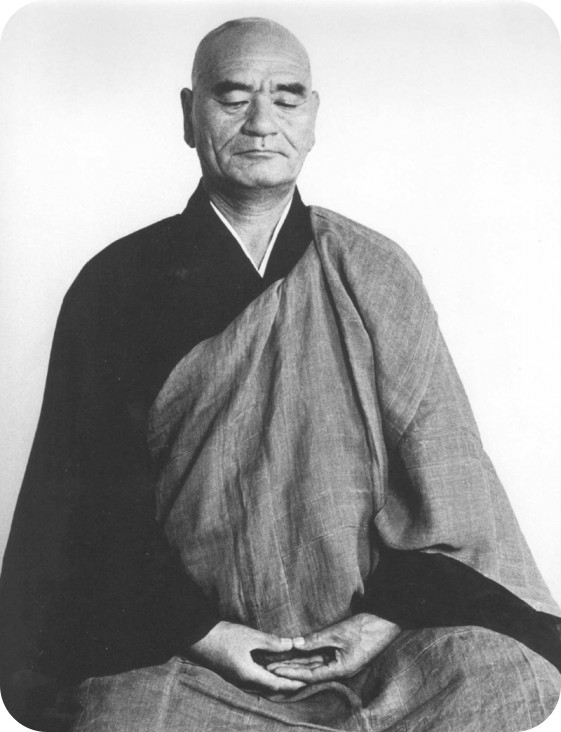
\includegraphics[width=0.7\linewidth]{figures/deshimaru}
\end{minipage}\begin{minipage}{0.7\columnwidth}
	\emph{\quotation{« Il faut dix minutes pour comprendre LaTeX, mais il faut toute une vie pour en maîtriser les pouvoirs. »}}
	\flushright{--- Deshimaru Sensei}
\end{minipage}
\end{figure}

\subsection{À l'origine du projet}

Le projet LaTeX a été lancé par Donald Knuth, un mathématicien de l'Université de Stanford. On lui doit, entre autres, la théorie de l'analyse des algorithmes et il est considéré comme l'un des pères de l'informatique moderne.

Par la suite, de nombreux contributeurs y ont ajouté des composants et de nombreuses fonctionnalités.
Il n'est donc pas développé par une entreprise comme Microsoft, mais par une communauté de développeurs qui l'améliorent selon leurs besoins. C'est aussi pour cette raison qu'il est gratuit.

\cadre{
\gr{Mais pourquoi personne ne l'utilise ?}\\
On ne vous a probablement pas parlé de LaTeX au collège, mais il y a quand même de nombreuses personnes qui s'en servent. Les scientifiques, en particulier dans les domaines de la physique et des mathématiques, utilisent généralement tous LaTeX. En effet, pendant longtemps, LaTeX a été le seul moyen d'écrire des équations correctement.\\
Il dispose aussi d'outils très perfectionnés pour gérer les citations bibliographiques, d'où sa popularité pour écrire des articles scientifiques.}

\section{De bonnes raisons pour l'utiliser}
Voyons quelques-uns des avantages que l'on peut avoir à utiliser LaTeX à la place de Word.

\subsection{Il est compatible avec tout}

Déjà, c'est un logiciel libre, gratuit et multi-plateforme. Cela veut dire qu'il fonctionnera partout, sur n'importe quel ordinateur, et que vous pouvez faire ce que vous voulez avec. Vous pouvez l'installer sur un ordinateur, mais il existe aussi des compilateurs en ligne où vous copiez-collez votre texte source dans un formulaire web, et ils vous renvoient votre document mis en forme au format pdf. Vous pourriez taper du LaTeX sur votre téléphone ou sur votre grille-pain, cela fonctionnera pareil. Il est même possible de l'utiliser depuis un smartphone.

Il n'affichera pas votre document n'importe comment sous prétexte que vous êtes sous Mac, ou que votre collègue utilise la version 2010 plutôt que 2011. Quand vous aurez utilisé LaTeX, vous serez étonné de vous rendre compte à quel point Word ne marchait pas.

\begin{tcolorbox}[breakable]
\gr{.doc, .odf et .docx}\\
À l'origine, Word utilisait le format \emph{.doc}. C'était un format propriétaire, c'est-à-dire que personne en dehors de Microsoft ne savait comment le lire, et on ne pouvait donc l'ouvrir qu'avec Word.\\

Puis, OpenOffice/LibreOffice sont apparus, avec leur propre format : le \emph{.odf}. Cette fois, il s'agit d'un format libre, avec toute la documentation nécessaire pour que les logiciels concurrents puissent le lire et le modifier comme ils le veulent.\\

Cela n'était pas à l'avantage de Microsoft, car si tout le monde commençait à utiliser le .odf, il n'y aurait plus de problèmes d'incompatibilité, et Microsoft perdraient leur monopole puisque chacun pourrait utiliser le logiciel qu'il souhaite.\\

Ils ont donc développé le format \emph{.docx}.
Il s'agit lui aussi d'un format libre, mais il est beaucoup plus compliqué que le format odf.
Sa documentation fait 6546 pages, il est donc presque impossible pour les concurrents de l'implémenter parfaitement.
Comme cela, Microsoft s'assurent que les problèmes persisteront et que leur monopole ne sera pas dérangé.
\end{tcolorbox}

Comme il est open-source, de nombreux outils ont pu être développés pour le travail collaboratif.
Nous en verrons quelques-uns à la section \ref{collab}, pour que vous puissiez travailler en équipe.

\subsection{Il donne des documents homogènes}

Avec LaTeX, vous vous contentez de dire « ça, c'est un titre », « ça, c'est une sous-section » et LaTeX s'occupe du reste.
Tous les titres auront donc la même apparence, la même police etc. Il n'est donc plus nécessaire de passer des heures à nettoyer le document pour que tout ait la même mise en forme (figure~\ref{clippy}).

\begin{figure}[h]
\centering\begin{minipage}{0.6\columnwidth}
	\caption{\emph{« Héhé... Il semblerait que vous soyez en train d'essayer de régler les marges de la page en bougeant les petits curseurs...~»}\label{clippy}}
\end{minipage}\hspace{5mm}\begin{minipage}{0.2\columnwidth}
	
\includegraphics[width=0.7\linewidth]{figures/clippy}
\end{minipage}
\end{figure}


\subsection{La numérotation}

Un autre avantage appréciable de LaTeX est qu'il sait compter. Que ce soient les numéros de parties, l'ordre des figures, les notes en pied de page ou les citations bibliographiques, il s'occupe de tout et vous n'aurez plus à vous préoccuper de la numérotation.

Si ces arguments vous ont donné envie de l'essayer, il ne vous reste plus qu'à l'installer.

\section{Installation}

\subsection{TeXLive}
LaTeX est un logiciel modulaire. Ce n'est pas un gros logiciel avec une liste de fonctionnalités déterminées. Il faut plutôt imaginer cela comme un noyau central, auquel s'ajoutent des milliers de petits modules indépendants qui ont chacun une fonction spécifique (il y a des modules pour écrire des partitions de musique, pour dessiner des formules chimiques ou encore pour décrire des parties d'échecs).

Si vous n'installiez que LaTeX tout seul, vous ne pourriez faire que le strict minimum. Et comme vous débutez, vous risqueriez d'avoir du mal à choisir les composants que vous voulez. Nous allons donc installer un kit qui contient tous les modules dont vous pourriez possiblement avoir besoin. Ce kit s'appelle TeXLive.

\subsubsection{Avec Linux}
Comme d'habitude, il suffit d'installer TeXLive avec le gestionnaire de logiciels. En général, le paquet s'appelle tout simplement \verb?texlive?.

\cadre{\gr{Sous Arch}, c'est \verb?texlive-most?, parce que les développeurs n'ont pas tout mis (ils ont par exemple retiré des packages qui servent à écrire en croate ou en arménien. Si vous les voulez vraiment, installez aussi \verb?texlive-lang?).}

\subsubsection{Avec Mac}
Nous allons installer MacTex, qui est une distribution gigantesque qui contient entre autres TexLive. Vous la trouverez ici :

\url{http://www.tug.org/mactex}

L'avantage, c'est que vous aurez \emph{tout} installé en un seul clic.

\subsubsection{Avec Windows}
Nous n'allons pas installer TexLive mais MiKTeX, une autre distribution similaire qui est plus légère. Cela ne devrait pas changer grand chose pour vous. Téléchargez MiKTeX ici :

\url{http://www.miktex.org}

Et suivez la marche à suivre décrite sur le site.

\subsection{Une interface digne de ce nom}
En théorie, n'importe quel logiciel capable d'écrire du texte suffit à créer des documents en LaTeX, puisque le code source n'est rien d'autre qu'un simple texte.
Cependant, il existe de très nombreux logiciels spécialement conçus pour écrire plus facilement vos documents.

Ces logiciels savent faire plusieurs choses très utiles~:
\begin{itemize}
	\item Compléter les commandes pour que vous n'ayez pas à les taper,
	\item Afficher un aperçu du pdf,
	\item Afficher les commandes en couleurs pour une meilleure lisibilité,
	\item Corriger l'orthographe,
	\item Afficher un sommaire pour se déplacer plus vite dans le document...
\end{itemize}

Nous allons en passer plusieurs en revue, il ne vous restera que l'embarras du choix. N'hésitez pas à en essayer plusieurs pour choisir votre préféré.

\subsubsection{Gummi}
Gummi est une interface pour LaTeX simple et très efficace. Elle permet d'afficher un aperçu en temps réel du document final, qui se met à jour dès que vous arrêtez de taper.

Gummi n'est hélas disponible que sous Linux.

\cadre{Maintenez Ctrl enfoncée et cliquez sur l'aperçu à l'endroit que vous voulez modifier. Cela vous emménera directement à l'endroit correspondant dans le code source.}

\subsubsection{TexShop}
TexShop est disponible sous Mac, et il est lui aussi très bien pour les débutants. Il est inclus dans MacTex, vous l'avez donc déjà installé. Si vous tapez le début d'une commande et que vous appuyez sur TAB, il cherchera à la compléter tout seul. Vous pouvez appuyer sur TAB jusqu'à trouver la bonne commande. C'est assez pratique.

\subsubsection{TexMaker}
TexMaker est assez similaire à Gummi. Il a l'avantage de fonctionner sur n'importe quel système d'exploitation.

\subsubsection{Lyx}

Cet éditeur est un peu spécial, car il reproduit le fonctionnement de Word, c'est-à-dire une interface avec des boutons. Avec Lyx, le code est masqué et les titres apparaissent directement en gros et en gras comme dans le document final. On perd donc une partie des avantages de LaTeX, mais il peut toujours dépanner si vous devez travailler avec quelqu'un qui ne sait pas se servir de LaTeX.

\subsubsection{Vim et Emacs}
Si vous êtes habitués à l'un de ces éditeurs de texte pour programmeurs, sachez qu'il est aussi possible de les utiliser pour écrire du LaTeX.

\subsection{Première compilation}
Pour bien comprendre le fonctionnement des choses, je vous propose de faire une première compilation à la main. Vous pouvez sans problème passer cette étape, car c'est un peu technique.

\begin{enumerate}
	\item Ouvrez un éditeur de texte brut (le bloc-note, gedit, nano...) et recopiez ceci sans vous tromper~:\begin{tcolorbox}[colback=white,colframe=black!50!white]
\begin{verbatim}
\documentclass[11pt]{article}
\begin{document}
Bonjour le monde.
\end{document}
\end{verbatim}

\end{tcolorbox}
	\item Sauvegardez ce fichier sous le nom test.tex
	\item Lancez un terminal et déplacez-vous à l'emplacement de test.tex
	\item Lancez la commande «~\verb?pdflatex test.tex?~»
	\item Regardez ce qui est apparu dans le dossier. En principe, il devrait y avoir entre autres un fichier pdf avec le texte «~Bonjour le monde.~».
\end{enumerate}
Et voilà, vous avec fait fonctionner LaTeX pour la première fois. Par la suite, c'est votre éditeur qui s'occupera de tout ça (ouf).

\subsection{Un modèle de document vide}
\begin{tcolorbox}[colback=white,colframe=black!50!white]
\begin{verbatim}
\documentclass[11pt]{article}

\usepackage[utf8]{inputenc}
\usepackage[T1]{fontenc}
\usepackage[french]{babel}

\begin{document}

\end{document}
\end{verbatim}
\end{tcolorbox}
Voici un modèle pour un document vide en français. Ce n'est pas grave si vous ne comprenez pas à quoi servent les trois \verb?\usepackage?, dites-vous simplement qu'ils permettent de gérer tous nos accents et autres bizarreries du français.

Gardez bien ce modèle sous la main, car nous allons l'utiliser tout le temps pour la suite de ce guide.\\

Le code source d'un document LaTeX est divisé en deux parties~:
\begin{itemize}
\item Tout ce qui se trouve avant \verb?\begin{document}? se nomme le \emph{préambule}.
C'est là que prendront place les réglages sur l'apparence et la mise en page du document.
\item Le vrai contenu du document sera à mettre entre \verb?\begin{document}? et \verb?\end{document}?.
\end{itemize}

La première ligne détermine la classe du document. Est-ce un article, un livre, une lettre ? Ici, nous utilisons la classe \verb?article?.

\cadre{\gr{La classe article}\\
En pratique, la classe «~article~» convient pour la plupart des documents courants. Nous allons nous y tenir dans ce guide.}

Maintenant que vous avez un modèle prêt à l'emploi, vous pouvez essayer de taper le texte de votre choix dans le corps du document, et de générer le pdf correspondant avec votre éditeur.

\section{Comment donner des instructions}
\subsection{Les commandes de LaTeX}
Avec LaTeX, toutes les instructions commencent par le signe \textbackslash. Cela s'appelle une contre-oblique (ou backslash). Ce n'est PAS un slash, il penche vers la gauche.

Quand LaTeX rencontrera ce caractère, il saura que vous voulez lui donner une indication sur ce qu'il doit faire.

Avec un clavier AZERTY, on obtient ce caractère avec AltGr + 8.
Souvenez-vous-en, vous allez en avoir besoin tout le temps.

\cadre{\gr{Si vous utilisez Mac}\\ Il faut taper « Alt + Majuscule + / ». Faites attention à ne pas abîmer vos ongles soigneusement manucurés en appuyant sur les touches.}

Un commande peut accepter différents paramètres (ou «~arguments~»).
Les arguments obligatoires s'écrivent entre accolades. Il s'agit en général du texte qui sera affecté par la commande.
Les arguments facultatifs s'écrivent entre crochets. Il permettent de faire des réglages, par exemple pour définir l'épaisseur d'un trait.

Voilà quelques exemples de ce à quoi une commande LaTeX complète peut ressembler :

\begin{figure}[h]
\centering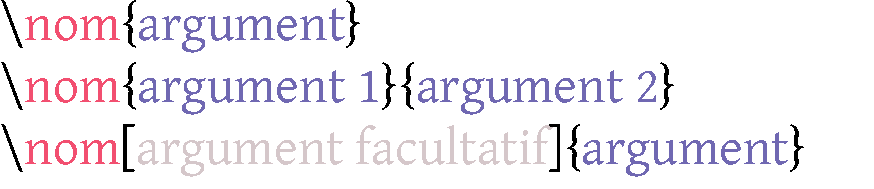
\includegraphics[width=0.4\linewidth]{figures/commandes}
\end{figure}

Mais il est temps pour vous d'apprendre votre première vraie commande : la commande \verb?\emph?.

La commande \verb?\emph{texte}? permet de faire une \emph{emphase} . Elle aura pour effet de mettre le texte entre accolades en italique.

\begin{tcolorbox}[colback=white,colframe=black!50!white]
\begin{verbatim}
Ceci est \emph{particulièrement} important.
\end{verbatim}
\end{tcolorbox}

Donnera : Ceci est \emph{particulièrement} important.

\section{La structure du document}

\subsection{Section, subsection, subsubsection} 
Nous allons voir les commandes que permettent de structurer le texte. Ce sont de loin les plus importantes.

\begin{itemize}
	\item \verb?\section{Titre de la section}? indique un titre de section.
	\item \verb?\subsection{Titre de la sous-section}? indique un titre de sous-section.
	\item \verb?\subsubsection{Titre de la sous-sous-section}? indique un titre de sous-sous-section.
\end{itemize}
Ce n'est pas si compliqué, n'est-ce pas ?

Maintenant, reprenez le modèle que je vous ai donné tout à l'heure, et écrivez ceci dans le corps du texte (c'est-à-dire dans la partie entre \verb?\begin{document}? et \verb?\end{document}?).
\begin{tcolorbox}[colback=white,colframe=black!50!white]
\begin{verbatim}
\section{Première partie}

\subsection{Sous-partie}
Contenu de la sous-partie.

\subsection{Autre sous-partie}
Contenu de la deuxième sous-partie.

\section{Deuxième partie}
Contenu de la deuxième grande partie.

\end{verbatim}
\end{tcolorbox}
Générez maintenant le pdf. Et voilà, remarquez comme LaTeX a tout pris en charge, et tout numéroté correctement.\\

Rien qu'avec ces différentes commandes, vous pouvez déjà faire la plupart de vos documents habituels. Évidemment, pour l'instant vous ne pourrez pas donner à votre article le design exact que vous imaginez, et vous devrez vous contenter du thème par défaut. Mais avec la pratique, vous progresserez petit à petit sans vous en rendre compte.

\subsection{Il faut vraiment taper tout ça à chaque fois ?}

Bien sûr que non. Il existe tout plein de méthodes pour ne pas avoir à
tout taper à la main. En fait, il n'est même pas nécessaire de se
souvenir d'une commande pour l'utiliser. Mais nous verrons ces méthodes
un peu plus tard dans le livre. Pour l'instant, vous êtes encore en
train d'apprendre, vous devrez donc taper les commandes en entier pour
bien comprendre comment ça fonctionne. Ensuite seulement, vous pourrez
chercher à gagner du temps en utilisant des raccourcis.

\subsection{Les «~environnements~»}

Ces commandes sont un peu particulières, puisqu'elles affectent non pas
ce qui est entre les accolades, mais tout ce qui se trouve entre les
deux commandes. On appelle cela un \emph{environnement}. Par exemple,
voici comment centrer du texte :

\begin{tcolorbox}[colback=white,colframe=black!50!white]
\begin{verbatim}
\begin{center}
Votre paragraphe centré ici.
\end{center}
\end{verbatim}
\end{tcolorbox}

Nous verrons d'autres environnements un peu plus tard.

\subsection{Faire des listes}

Faire des listes en LaTeX s'avère beaucoup moins aléatoire qu'avec Word.
En LaTeX, les listes sont des environnements.
Les trois principaux sont \verb?itemize?, \verb?enumerate? et \verb?description?, ils correspondent aux trois types de liste les plus communs.
À l'intérieur de l'environnement, on écrit les items de la liste avec la commande \verb?\item?.

Mais quelques exemples valent mieux qu'une longue explication :

\subsubsection{Itemize}
Une liste normale, avec des tirets.

\noindent\begin{minipage}{0.45\columnwidth}
\begin{tcolorbox}[colback=white,colframe=black!50!white]
\begin{verbatim}
\begin{itemize}
	\item Premier item,
	\item Deuxième item,
	\item Troisième item.
\end{itemize}
\end{verbatim}
\end{tcolorbox}
\end{minipage}\hfill\begin{minipage}{0.4\columnwidth}
\begin{itemize}
	\item Premier item,
	\item Deuxième item,
	\item Troisième item.
\end{itemize}
\end{minipage}

\subsubsection{Description}
Celle-là permet d'écrire des définitions, comme dans un dictionnaire.

\noindent\begin{minipage}{0.45\columnwidth}
\begin{tcolorbox}[colback=white,colframe=black!50!white]
\begin{verbatim}
\begin{description}
	\item[Mot :] Définition,
	\item[Mot :] Définition,
	\item[Mot :] Définition.
\end{description}
\end{verbatim}
\end{tcolorbox}
\end{minipage}\hfill\begin{minipage}{0.36\columnwidth}
\begin{description}
	\item[Mot :] Définition,
	\item[Mot :] Définition,
	\item[Mot :] Définition.
\end{description}
\end{minipage}

\subsubsection{Enumerate}
Enfin, \emph{enumerate} sert à faire des listes numérotées.

\noindent\begin{minipage}{0.45\columnwidth}
\begin{tcolorbox}[colback=white,colframe=black!50!white]
\begin{verbatim}
\begin{enumerate}
	\item Premier item,
	\item Deuxième item,
	\item Troisième item.
\end{enumerate}
\end{verbatim}
\end{tcolorbox}
\end{minipage}\hfill\begin{minipage}{0.4\columnwidth}
\begin{enumerate}
	\item Premier item,
	\item Deuxième item,
	\item Troisième item.
\end{enumerate}
\end{minipage}

\subsection{La page de titre}

Avant de créer un titre, nous allons déjà donner au logiciel les informations nécessaires, en écrivant les commandes suivantes dans le préambule~:

\begin{tcolorbox}[colback=white,colframe=black!50!white]
\begin{verbatim}
\title{Votre titre}
\author{Votre nom}
\date{La date}
\end{verbatim}
\end{tcolorbox}
Si vous ne mettez pas la commande \verb?\date?, la date d'aujourd'hui sera utilisée.

Ensuite, à l'endroit où vous voulez placer votre titre, utilisez la commande \verb?\maketitle?. Cela fera apparaître un grand titre.

Cette commande permet de créer un titre simple et élégant, mais elle ne permet pas beaucoup de customisation. Si vous voulez faire un titre plus sophistiqué, mieux vaut le faire à la main et ne pas du tout utiliser \verb?\maketitle?.

\subsection{Faire des paragraphes}
Les retours à la ligne simples ne sont pas pris en compte par LaTeX.
Vous pouvez donc aérer votre code source.
Beaucoup de gens appuient sur Entrée après chaque phrase, voire après chaque idée distincte.
C'est un bon moyen d'avoir les idées plus claires.

\noindent\begin{minipage}{0.4\columnwidth}
\begin{tcolorbox}[colback=white,colframe=black!50!white]
\begin{verbatim}
Aaa
Bbb
Ccc.
\end{verbatim}
\end{tcolorbox}
\end{minipage}\hfill\begin{minipage}{0.5\columnwidth}
Aaa
Bbb
Ccc.
\end{minipage}

Par conséquent, pour avoir un \emph{retour à la ligne} dans le document, il faut \emph{passer une ligne} dans le code source.

\noindent\begin{minipage}{0.4\columnwidth}
\begin{tcolorbox}[colback=white,colframe=black!50!white]
\begin{verbatim}
Aaa.

Bbb.
\end{verbatim}
\end{tcolorbox}
\end{minipage}\hfill\begin{minipage}{0.5\columnwidth}
Aaa.

Bbb.
\end{minipage}

Le double-antislash \textbackslash\textbackslash{} donne le même résultat.

\noindent\begin{minipage}{0.4\columnwidth}
\begin{tcolorbox}[colback=white,colframe=black!50!white]
\begin{verbatim}
Aaa.\\
Bbb.
\end{verbatim}
\end{tcolorbox}
\end{minipage}\hfill\begin{minipage}{0.5\columnwidth}
Aaa.\\
Bbb.
\end{minipage}

Mais alors, comment passer une ligne dans le document~?
Il suffit d'utiliser la commande \textbackslash\textbackslash{} puis de passer une ligne dans le code source. Cela peut paraître un peu confus, mais on s'y habitue.

\noindent\begin{minipage}{0.4\columnwidth}
\begin{tcolorbox}[colback=white,colframe=black!50!white]
\begin{verbatim}
Aaa.\\

Bbb.
\end{verbatim}
\end{tcolorbox}
\end{minipage}\hfill\begin{minipage}{0.5\columnwidth}
Aaa.\\

Bbb.
\end{minipage}









\subsection{Charger des packages}
Les packages, ce sont comme des extensions qui vous permettent de vous simplifier la vie. Avant de s'en servir, il faut dire à LaTeX que l'on veut l'utiliser en écrivant cette commande \emph{dans le préambule} (avant \verb?\begin{document}?):
\begin{tcolorbox}[colback=white,colframe=black!50!white]
\begin{verbatim}
\usepackage{nom du package}
ou bien
\usepackage[options]{nom du package}
\end{verbatim}
\end{tcolorbox}
Certains package prennent effet dès qu'on les appelle (essayez avec le package \verb?cmbright?, qui change l'apparence du texte) :

\begin{tcolorbox}[colback=white,colframe=black!50!white]
\begin{verbatim}
\usepackage{cmbright}
\end{verbatim}
\end{tcolorbox}

D'autres rendent disponibles de nouvelles commandes (par exemple \verb?chemfig? donne accès à des commandes pour écrire des formules chimiques).

\begin{tcolorbox}[colback=white,colframe=black!50!white]
\begin{verbatim}
\usepackage{chemfig}
\end{verbatim}
\end{tcolorbox}

Puis, dans le corps du document, essayez par exemple d'écrire ceci : 

\begin{tcolorbox}[colback=white,colframe=black!50!white]
\begin{verbatim}
\chemfig{HOOC-*6(-=-=-=)}
\end{verbatim}
\end{tcolorbox}
Vous obtiendrez une belle molécule d'acide benzoïque.



\section{Des images, des figures et des tableaux}

\subsection{Des images}
Commencez par charger le package \emph{graphicx} dans le préambule (\verb?\usepackage{graphicx}?).\\

La commande pour inclure une image est \verb?\includegraphics?. 
Entre les accolades, il faut écrire le nom du fichier de l'image, qui doit se trouver dans le même dossier que le fichier tex. 
Les formats d'image reconnus sont png, jpg, pdf et eps. 
Il n'est pas nécessaire d'écrire l'extension du nom de fichier : 
si plusieurs images portent le même nom dans des formats différents, LaTeX choisira la meilleure.

Par exemple, si vous mettez une image nommée lapin.png à côté de votre fichier tex, voici comment l'afficher :
\begin{tcolorbox}[colback=white,colframe=black!50!white]
\begin{verbatim}
\includegraphics{lapin}
\end{verbatim}
\end{tcolorbox}

Le nom du fichier ne doit pas contenir d'espace, utilisez plutôt des traits d'union (petit-lapin.jpg).

Vous pouvez régler les dimensions de l'image en utilisant les paramètres \verb?width? et \verb?height?. Attention, si vous mentionnez les deux l'image apparaîtra déformée.

\begin{tcolorbox}[colback=white,colframe=black!50!white]
\begin{verbatim}
\includegraphics[width=40mm]{lapin}
\includegraphics[height=30mm]{lapin}

\includegraphics[width=40mm,height=30mm]{lapin}
\end{verbatim}
\end{tcolorbox}
N'oubliez pas de mettre une unité (mm, cm, px...). Pour les nombres décimaux, il faut mettre un point à la place de la virgule (\verb?width=4.2cm? par exemple).

Une commande très utile à ce moment est \verb?\linewidth?, qui correspond à la largeur du texte. Vous pouvez mettre un coefficient avant : \verb?0.5\linewidth? correspond à la moitié d'une ligne, par exemple.

\begin{tcolorbox}[colback=white,colframe=black!50!white]
\begin{verbatim}
\includegraphics[width=\linewidth]{lapin}
\includegraphics[width=0.5\linewidth]{lapin}
\end{verbatim}
\end{tcolorbox}

\subsubsection*{Images vectorielles ou matricielles ?}
Puisque nous parlons d'inclure des images, voici un conseil important (qui est valable aussi avec Word/Writer). Vous devriez utiliser des images \emph{vectorielles}. 

Les images que vous avez l'habitude d'utiliser (jpg, png, etc.) enregistrent la couleur de chaque pixel. On dit qu'elles sont \emph{matricielles}.

Au contraire, les images vectorielles enregistrent la forme, la couleur et l'épaisseur des traits. Les principaux formats sont \emph{pdf}, \emph{svg} et \emph{eps}. L'avantage, c'est que l'on peut changer leur taille n'importe comment, la qualité restera la même. Le résultat sera par conséquent bien meilleur à l'impression (figure \ref{vect}). Les images vectorielles sont aussi bien plus légères.

\begin{figure}[h]
\centering
\includegraphics[height=95px]{figures/cah.pdf}
\includegraphics[height=95px]{figures/cah.png}

\caption{\emph{La même image en vectoriel (gauche) et en matriciel (droite). Essayez de zoomer dessus, vous verrez la différence.}}
\label{vect}
\end{figure}

Un bon logiciel pour faire vos schémas en vectoriel est \emph{Inkscape}. Sinon, il y a Adobe Illustrator. Excel et Calc permettent d'exporter leurs graphiques en vectoriel, au format pdf. Notez que LaTeX ne connaît pas le svg, si vous en avez il faudra le convertir en pdf.

\cadre{Préférez toujours des images vectorielles, quand c'est possible.}

\subsection{Des tableaux}\label{tableaux}

Autant vous prévenir tout de suite, les commandes de LaTeX pour faire des tableaux sont un peu compliquées. 
Plutôt que des les construire à la main, je vous conseille de les générer automatiquement :
\begin{itemize}
	\item Vous pouvez par exemple utiliser un éditeur de tableaux en ligne, tel que l'excellent 

\url{www.tablesgenerator.com/}
	\item Il existe des plug-ins pour exporter du code LaTeX depuis Excel, LibreOffice et même R. Il suffit de le googler.
	\item Regardez dans votre éditeur LaTeX, la plupart possèdent des outils pour construire des tableaux (avec Gummi, le bouton se trouve en bas à gauche).
\end{itemize}

Un exemple de ce que ça donne~:

\noindent\begin{minipage}{0.5\columnwidth}
\begin{tcolorbox}[colback=white,colframe=black!50!white]
\begin{verbatim}
\begin{tabular}{|l|l|l|}
\hline
	Voici & Le & Type\\
\hline
	De & Code & Que\\
\hline
	Vous & Allez & Obtenir\\
\hline
\end{tabular}
\end{verbatim}
\end{tcolorbox}
\end{minipage}\hfill\begin{minipage}{0.4\columnwidth}
\begin{tabular}{|l|l|l|}
\hline
	Voici & Le & Type\\
\hline
	De & Code & Que\\
\hline
	Vous & Allez & Obtenir\\
\hline
\end{tabular}
\end{minipage}

\cadre{Si vous voulez comprendre comment tout cela fonctionne, c'est ici :\\ \url{https://fr.wikibooks.org/wiki/LaTeX/Tableaux}.}

\subsection{Les figures}
Tout cela est très bien, mais vous n'allez tout de même pas balancer vos images et vos tableaux en plein milieu du texte comme des barbares.

Nous allons les mettre dans des \emph{flottants}. Le principe d'un flottant, c'est qu'il flotte. Le contenu du flottant n'apparaîtra pas directement là où vous l'avez mis : LaTeX va plutôt chercher le meilleur endroit pour le caser à proximité, en général entre deux paragraphes. Vous pourrez ensuite l'appeler dans le texte en disant par exemple «~voir figure~1~». Vous pourrez aussi générer facilement une liste des figures et une liste des tables, dans le cas d'un mémoire.

Pour faire un flottant, il suffit d'utiliser l'environnement \verb?figure? pour les images, et \verb?table? pour les tableaux.

\begin{tcolorbox}[colback=white,colframe=black!50!white]
\begin{verbatim}
\begin{figure}[h]
\includegraphics[width=\linewidth]{votre-image}
\end{figure}
\end{verbatim}
\end{tcolorbox}
Le petit \verb?[h]? sert à indiquer à quel endroit vous voulez que le flottant soit. [h] signifie \emph{here}, donc LaTeX le placera le plus près possible de l'endroit où la commande est écrite.

Les autres possibilités sont [t] (\emph{top}, en haut de la page), [b] (\emph{bottom}, en bas) et [p], qui indique à LaTeX de faire une page à part où il mettra toutes les figures.  
 
 Pour les tableaux, c'est exactement le même fonctionnement. Il suffit de remplacer le mot \verb?figure? par \verb?table?.
 
\subsubsection{Une légende}
La commande \verb?\caption{votre légende ici}? permet d'ajouter une légende. Placez là quelque part dans le flottant.
\cadre{Par convention, vous devez placer la légende en dessous pour une image, et au dessus pour un tableau.}
\subsubsection{Appeler une figure dans le texte}
Et maintenant, le plus difficile : faire référence à une figure dans le texte. Nous allons faire cela grâce à deux commandes qui vont ensembles, \verb?\label? et \verb?\ref?.

Ces commandes fonctionnent avec des mots clés.
En mettant \verb?\label{mot-clé}? dans la figure, vous définissez un mot clé associé à une figure précise.
En mettant \verb?\ref{mot-clé}? dans le texte, vous récupérez le numéro de la figure correspondant. Voyons un exemple~:

\begin{tcolorbox}[colback=white,colframe=black!50!white]
\begin{verbatim}
\begin{figure}[h]

UNE PHOTO DE PINGOUIN
\caption{Votre légende.}
\label{pingouin}

\end{figure}

...comme on peut le voir sur la figure \ref{pingouin}.
\end{verbatim}
\end{tcolorbox}

\cadre{Il faut générer le pdf deux fois de suite pour que ces commandes fonctionnent.}

\cadre{Ces deux commandes ne sont pas limitées aux figures. Utilisées ailleurs, elles permettent de renvoyer à une section particulière.}


\section{D'autres commandes indispensables}

\subsection{Écrire des commentaires dans le code source}

En LaTeX, le caractère \% permet d'insérer des commentaires dans le code. Tout ce qui se trouve après ce caractère jusqu'à la fin de la ligne ne sera pas pris en compte lors de la compilation du document.

Utilisez les commentaires pour laisser des petits messages cachés aux personnes avec qui vous travaillez.

\subsection{Note en pied de page}

La commande \verb?\footnote{Votre note ici}? permet d'écrire des notes en pied de page\footnote{Comme cela.}. Il suffit de l'insérer à l'endroit voulu dans le texte, LaTeX se charge de la numérotation tout seul\footnote{Voyez plutôt.}.

\subsection{Quelques caractères spéciaux}

\subsubsection{Pourcentages}
Nous avons vu que \% servait à écrire des commentaires. Si vous voulez
parler d'un pourcentage, utilisez la commande \verb?\%? qui permet
d'obtenir ce caractère comme si de rien n'était.

\subsubsection{Dollars et euros}
De même, \verb?$? sert à écrire des formules de maths, il faut donc
utiliser la commande \verb?\$? pour afficher la caractère \$ dans un
texte. Pour les euros, c'est la commande \verb?\euro?, qui nécessite
d'abord d'importer le package \emph{eurosym}.

\subsubsection{Lettres grecques}
Pour taper des lettres grecques, c'est un peu compliqué. Il faut
importer le package \emph{upgreek} dans le préambule, puis taper \verb?$\upalpha$?,
\verb?$\upbeta$?, \verb?$\upgamma$? etc. Pour les lettres grecques
majuscules, c'est la même chose mais avec une majuscule, par exemple
\verb?$\Updelta$?.

\cadre{Il faut entourer la commande avec des \$ car, à l'origine, ces lettres sont censées être utilisées dans des formules de maths. Les développeurs de LaTeX n'ont manifestement jamais eu à écrire un texte sur les récepteurs de l'adrénaline.}

\subsection{Numéros de page}\label{numuxe9ros-de-page}

\begin{itemize}
\item \verb?\thispagestyle{empty}? enlève le numéro de la page où la commande est invoquée,
\item \verb?\pagestyle{empty}? enlève tout bonnement les numéros de page de tout de le document, à partir de la commande.
\end{itemize}

\subsection{Écrire en exposant}
La commande pour écrire «~en haut~» est \verb?\up{...}?.

\noindent\begin{minipage}{0.5\columnwidth}
\begin{tcolorbox}[colback=white,colframe=black!50!white]
\begin{verbatim}
1\up{er}, 2\up{e}, 3\up{e}.
\end{verbatim}
\end{tcolorbox}
\end{minipage}\hfill\begin{minipage}{0.4\columnwidth}
1\up{er}, 2\up{e}, 3\up{e}.
\end{minipage}

\subsection{Et pour aller plus loin...}

Si vous êtes habitué à Word, vous vous demandez sûrement « comment on fait pour changer la couleur d'un mot », « comment on change la police d'une phrase » et autres questions du même genre.
En vérité, on a rarement besoin de faire ce genre de chose quand on écrit un document sérieux. Mais si vous voulez vraiment le faire, regardez ici :

\url{https://fr.wikibooks.org/wiki/LaTeX/Mise_en_forme_du_texte}






\section{L'apparence du document}

\subsection{Vous avez probablement tort}

Il est bien sûr possible de customiser chaque pixel de vos documents, mais c'est rarement une bonne idée. LaTeX fait des documents très classiques, qui respectent les standards de la typographie et de l'imprimerie. N'oubliez jamais ceci :
\emph{Le style par défaut convient.}

Vous pouvez le changer, mais vous allez y passer du temps et le résultat sera probablement moins bien qu'au départ.

\cadre{\gr{Un exemple de chose à ne pas faire}\\
La commande \texttt{textbf} permet de mettre du texte en gras. Cependant, les titres seront déjà mis en caractères gras automatiquement, et il est typographiquement incorrect d'utiliser du gras en plein paragraphe. Vous n'aurez donc jamais besoin d'employer cette commande en pratique.

Mais allez faire comprendre cela à un utilisateur de Word.}

Voici quand même quelques réglages qui pourront se révéler utiles dans certaines situations.

\subsection{Taille du texte}

Certains réglages qui concernent tout le document prennent place dès la première ligne du code, entre les crochets de la commande \verb?\documentclass?.

Les paramètres possibles sont \verb?10pt?, \verb?11pt? et \verb?12pt?. Exemple :
\begin{tcolorbox}[colback=white,colframe=black!50!white]
\verb?\documentclass[11pt]{article}?
\end{tcolorbox}
 Les autres tailles ne sont pas disponible par cette méthode. En règle générale, si LaTeX ne veut pas faire quelque chose, c'est qu'il ne faut pas le faire.

\subsection{La police d'écriture}\label{police}
En règle générale, on préfère utiliser une seule et unique police pour l'ensemble du document, que ce soit pour les titres, les équations ou les légendes de schémas. Nous allons donc utiliser des packages spéciaux qui changent uniformément la police de tout le document.
Par exemple, ajouter \verb?\usepackage{times}? dans le préambule mettra tout le document en Times New Roman.

Par conséquent, seules les polices permettant d'écrire des équations mathématiques sont disponibles sous forme de packages. Mais rassurez-vous, il existe suffisamment de packages pour couvrir tous vos besoins.

Voici quelques autres packages de polices incluses dans TeXLive~:
\begin{itemize}
	\item \verb?mathpazo? : Correspond à la police \emph{Palatino}. Très bien pour un document à imprimer.
	\item \verb?cmbright? : Une police sans sérif très lumineuse.
	\item \verb?concmath? : Une police assez vintage.
	\item \verb?gentium? : C'est la police que vous avez devant les yeux.
\end{itemize}
Vous pourrez trouver un catalogue de polices d'écriture avec les packages correspondants ici :\\
\url{http://www.tug.dk/FontCatalogue}

\cadre{\gr{Et le Comic Sans MS ?}\\
Quelqu'un s'est amusé à créer un package pour cela, mais il n'est pas inclus dans TexLive. Vous devrez donc l'installer vous-même pour connaître le plaisir d'écrire des équations mathématiques en Comic Sans MS.\\
\url{http://www.ctan.org/tex-archive/fonts/comicsans}}

\subsection{Géometrie}
Le package \verb?geometry? permet de faire tous les réglages imaginables par rapport à la taille des marges, du papier, des colonnes, et bien plus encore. Voici quelques exemples.

Donner à toutes les marges une largeur de 20~mm avec \verb?margin=?~:
	\begin{tcolorbox}[colback=white,colframe=black!50!white]
	\begin{verbatim}
	\usepackage[margin=20mm]{geometry}
	\end{verbatim}
	\end{tcolorbox}
Régler chaque marge séparément avec \verb?top,bottom,right? et \verb?left?~:
	\begin{tcolorbox}[colback=white,colframe=black!50!white]
	\begin{verbatim}
	\usepackage[top=5px,bottom=5px]{geometry}
	\end{verbatim}
	\end{tcolorbox}

N'oubliez pas de mettre une unité aux longueurs.

\subsection{Domptez LaTeX}

Pour finir, voilà quelques commandes extrêmement utiles. Elles permettent de régler finement la position des différents élements, dans le cas ou LaTeX ne les aurait pas placés au bon endroit.

\vspace{3mm}\verb?\vspace{15mm}? laisse un espace vide vertical de la longueur souhaitée. Vous pourrez donc régler au millimètre près la distance entre deux paragraphes, etc. En mettant une longueur négative, vous pouvez aussi remonter un élément.

\vspace{3mm}\verb?\hspace{15mm}? correspond à un espace horizontal.

\vspace{3mm}\verb?\hfill? pousse ce qui se trouve après lui au maximum vers la droite. Exemple :

\begin{tcolorbox}[colback=white,colframe=black!50!white]
\verb?À gauche.\hfill À droite. ?
\end{tcolorbox}

À gauche.\hfill À droite

\vspace{3mm}\verb?\noindent? supprime l'indentation si vous le mettez au début d'un paragraphe ou avant une image.

\vspace{3mm}\verb?\clearpage? permet de continuer faire un saut de page.

\section{Comment aller plus vite}
Les commandes de LaTeX sont souvent un peu longues à taper.
Heureusement, les éditeurs permettent de gagner du temps en les complétant pour vous.

\subsection{Les \emph{snippets} }
Globalement, tous les éditeurs fonctionnent de la même façon.
Vous commencez à taper une commande, vous appuyez sur TAB, et l'éditeur rajoute la fin.
La plupart des éditeurs permettent de créer vos propres raccourcis, de sorte que vous n'ayez qu'à taper un mot d'appel puis appuyer sur TAB, et le logiciel rajoute une section de code définie à l'avance.
Par exemple, vous pourrez faire en sorte que, si vous écrivez «~fig~» puis appuyez sur TAB, le code suivant tout entier apparaisse :

\begin{tcolorbox}[colback=white,colframe=black!50!white]
\begin{verbatim}
\begin{figure}
	\includegraphics[width=\linewidth]{}
	\caption{}
	\label{}
\end{figure}
\end{verbatim}
\end{tcolorbox}

Et vous n'aurez plus qu'à compléter les différents éléments.
Il faut reconnaître que c'est assez pratique, surtout que cela évite de mémoriser les commandes les plus compliquées.
N'hésitez pas à fouiller dans votre éditeur pour trouver les options correspondantes.

\cadre{\gr{Avec Gummi}, c'est particulièrement simple.
Vous pouvez créer des \emph{snippets} de ce genre en allant dans Édition / Préférences / Éditeur / Configurer les extraits de code.
Vous pouvez alors choisir un mot d'appel et écrire le code correspondant. 
Insérez ensuite des repères «~\$1~», «~\$2~», «~\$3~» et ainsi de suite à l'emplacement des différents élements à compléter. 
Quand vous utiliserez votre \emph{snippet}, vous n'aurez qu'à appuyer sur TAB à nouveau pour passer de l'un à l'autre et remplir rapidement tous les champs.}

\subsection{D'autres langages et des convertisseurs}
Une autre façon de procéder est de rédiger votre document en utilisant un autre langage descriptif plus simple que LaTeX. 
Il en existe plein, je vous conseille particulièrement Markdown ou Mediawiki (qui est la syntaxe utilisée pour écrire des articles de Wikipédia), car ils sont très faciles à apprendre.

Quand vous aurez écrit votre document, il vous suffira d'utiliser un convertisseur comme Pandoc, qui le traduira automatiquement en LaTeX.
Il existe de nombreux autres convertisseurs, je vous laisse faire votre choix.


Pandoc fonctionne en ligne de commande, pour convertir un fichier de mediawiki vers LaTeX il faut taper ceci dans un terminal~:

\begin{tcolorbox}[colback=white,colframe=black!50!white]\verb?pandoc -f mediawiki -t latex votre_fichier?\end{tcolorbox}

\noindent\begin{minipage}{0.49\columnwidth}
\begin{tcolorbox}[colback=white,colframe=black!50!white]
\gr{Version originale (mediawiki)}
\begin{verbatim}
=Section=
==Sous-section==
Liste :
*a
*b
*c


\end{verbatim}
\end{tcolorbox}
\end{minipage}\hfill\begin{minipage}{0.49\columnwidth}
\begin{tcolorbox}[colback=white,colframe=black!50!white]
\gr{Version LaTeX après conversion}
\begin{verbatim}
\section{Section}
\subsection{Sous-section}
Liste :
\begin{itemize}
\item a
\item b
\item c
\end{itemize}
\end{verbatim}
\end{tcolorbox}
\end{minipage}

Le code mediawiki est quand même bien plus simple et plus lisible. 
Cela peut d'ailleurs être un bon moyen de convaincre vos collaborateurs de faire des documents en LaTeX.





\section{Travailler en groupe}\label{collab}
Maintenant que vous savez rédiger des documents en LaTeX, vous serez sans doute amenés à travailler avec d'autres personnes sur un même document. Heureusement, il existe plein de façons différentes de le faire et vous devriez en trouver une qui convient à vos collègues (même s'ils ne connaissent pas très bien LaTeX).

\subsection{ShareLaTeX}
Voici un outil que je vous recommande fortement si vous souhaitez travailler à plusieurs. Il s'agit d'un éditeur LaTeX en ligne, qui fonctionne exactement comme Google Docs, mais avec LaTeX.

Vous le trouverez à cette adresse : \url{www.sharelatex.com}\\

Il vous permet de travailler à plusieurs en même temps sur un même fichier (vous voyez en direct les modifications de vos collègues). ShareLaTeX comprend aussi un compilateur en ligne (basé sur TeXLive) qui permet de télécharger le fichier pdf final même sur un ordinateur où LaTeX n'est pas installé.

Bref, ShareLaTeX c'est bien.

\subsection{Input et Subfiles}
La commande \verb?\input? permet tout simplement de récupérer le contenu d'un autre fichier texte, et de le mettre à la place de \verb?\input?.

\begin{tcolorbox}[colback=white,colframe=black!50!white]
\begin{verbatim}
\input{autre-fichier.tex}
\end{verbatim}
\end{tcolorbox}

Ainsi, vous pouvez par exemple mettre le préambule, la bibliographie ou les figures dans un fichier séparé, de façon à vous y retrouver plus facilement.
Si vous travaillez sur un projet ou chaque personne doit rédiger une section, vous pouvez faire un fichier général qui ne contiendra que le préambule et des \verb?\input? vers les différentes parties.
Chaque personne pourra alors travailler parallèment sur sa partie, sans qu'il y a ait besoin de gérer les différentes versions du document final.

Mieux encore, le package \verb?subfiles? est spécialement prévu pour le travail en groupe. Il fonctionne d'une façon similaire à \verb?\input?, mais permet de compiler les sous-fichiers indépendamment pour avoir un aperçu.

\begin{tcolorbox}[colback=white,colframe=black!50!white]
\gr{fichier-principal.tex}
\begin{verbatim}
\usepackage{subfiles}

\begin{document}

\subfile{fichier-secondaire1.tex}
\subfile{fichier-secondaire2.tex}
\subfile{fichier-secondaire3.tex}

\end{document}
\end{verbatim}
\end{tcolorbox}

\begin{tcolorbox}[colback=white,colframe=black!50!white]
\gr{fichier-secondaire1.tex}
\begin{verbatim}
\documentclass[fichier-principal.tex]{subfiles}

\begin{document}

\section{La première section}
Contenu de la section.

\end{document}
\end{verbatim}
\end{tcolorbox}

\subsection{Git, Subversion...}
Ces logiciels sont beaucoup utilisés par les développeurs de logiciels pour travailler à plusieurs sur un seul code source. 
Ils sont tout à fait adaptés pour LaTeX et vous pouvez vous en servir. 
En revanche, si vous n'êtes pas informaticiens il y a peu de chances pour que vos collègues soient prêt à s'en servir...

\section{Aller plus loin}
Pour finir, voici quelques informations qui ne vous seront peut-être pas utiles tout de suite, mais qui pourront le devenir quand vous serez habitués à LaTeX.

\subsection{Une table des matières incluse dans le pdf}
Certains lecteurs de pdf permettent d'afficher un sommaire dans un panneau, de façon à pouvoir naviguer dans le document en cliquant sur les titres de sections. Pour cela, il faut d'abord que le sommaire en question soit inclu dans le pdf sous forme de \emph{méta-données}. Avec LaTeX, il suffit d'utiliser le package \verb?hyperref? avec l'option \emph{hidelinks}. 

\begin{tcolorbox}[colback=white,colframe=black!50!white]
\begin{verbatim}
\usepackage[hidelinks]{hyperref}
\end{verbatim}
\end{tcolorbox}

\cadre{Le package \emph{hyperref} sait aussi faire tout plein de bonnes choses, comme faire fonctionner les liens hypertextes, rendre cliquable la table des matières, etc. N'hésitez pas à l'utiliser.}

\subsection{Corriger les fautes}
Pour corriger l'orthographe de votre document, il y a souvent un correcteur inclus dans votre éditeur.
Mais ces correcteurs ne sont en général pas très avancés, et il peut être utile de vérifier votre document avec un outil plus élaboré. 
Pour cela, nous allons d'abord enlever tout le code LaTeX, pour ne garder que le texte.

Cela peut se faire facilement en utilisant un script comme \verb?opendetex? :

\url{code.google.com/p/opendetex}\\

Écrivez «~\verb?detex votre_fichier?~» dans un terminal pour obtenir le texte brut.
Maintenant, vous pouvez chercher les fautes avec l'outil de votre choix~:

\url{www.reverso.net/orthographe/correcteur-francais}

\url{www.bonpatron.com}

Vous pouvez même copier-coller votre texte dans Word, après vous être assuré que personne ne vous regarde.

\subsection{Des commandes personnalisées}
La commande \verb?\newcommand? sert à créer vos propres commandes.
C'est très pratique, car cela vous permet de remplacer une série de commandes compliquées par une seule commande simple.
Elle prend deux arguments : d'abord le nom de votre nouvelle commande (n'oubliez pas de commencer par un \textbackslash{}), et ensuite la série de commandes à remplacer.
Par exemple, si vous n'avez pas envie de taper \verb?$\upmu$? à chaque fois que vous écrivez une quantité en microlittres, vous pouvez créer une commande pour cela~:

\noindent\begin{minipage}{0.52\linewidth}
\begin{tcolorbox}[colback=white,colframe=black!50!white]
\begin{verbatim}
\newcommand{\ul}{ $\upmu$l }

Prélevez 5\ul de solution.
\end{verbatim}
\end{tcolorbox}
\end{minipage}\hfill\begin{minipage}{0.43\linewidth}
\newcommand{\ul}{~$\upmu$l }

Prélevez 5\ul de solution.
\end{minipage}

En fait, il est possible de programmer des commandes beaucoup plus complexes, vous trouverez tous les détails pour cela ici :

\url{https://en.wikibooks.org/wiki/LaTeX/Macros}

\subsection{Créer des diaporamas}
Il est possible de faire des diaporamas impeccables avec LaTeX, en utilisant la classe \verb?beamer? (figure~\ref{beamer}).
Je ne vais pas m'étendre sur le sujet, l'Internet est déjà parsemé de tutoriels à ce propos.

\begin{figure}[h]
\centering\tcbox[boxsep=0pt]{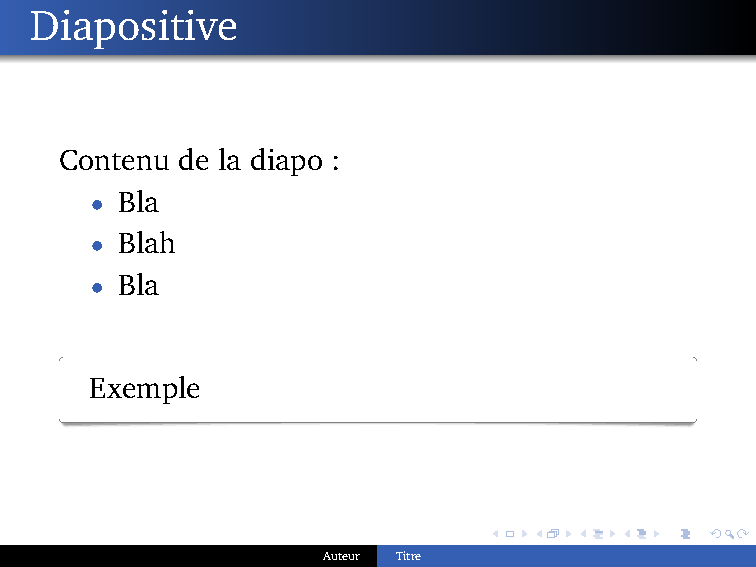
\includegraphics[width=0.4\linewidth]{figures/beamer}}
	\caption{Un exemple de diapositive créée avec Beamer.}
	\label{beamer}
\end{figure}

Le principal avantage de Beamer, c'est qu'il permet de gagner énormément de temps quand on a un peu l'habitude de travailler avec LaTeX.
Si vous savez quoi écrire, votre diaporama sera prêt en quelques minutes.

\cadre{\gr{qpdfpresenterconsole}\\
Quand on utilise PowerPoint, il est possible de présenter un diaporama sur un projecteur, tout en affichant sur votre ordinateur un aperçu de la diapo suivante, un chronomètre, et d'autres éléments utiles.
Le logiciel qpdfpresenterconsole permet de faire la même chose avec des diaporamas en pdf, ce qui en fait un outil génial si vous utilisez Beamer.
}

Ainsi s'achève cette introduction à LaTeX.
Ce n'est qu'une introduction, pour que vous puissiez rapidement faire vos premiers projets sans faire n'importe quoi.
Si vous voulez en savoir plus sur une commande ou une autre, vous pourrez trouver toutes sortes d'informations détaillées sur \url{en.wikibooks.org/wiki/LaTeX} (en anglais) ou \url{fr.wikibooks.org/wiki/LaTeX} (en français).
N'oubliez pas que c'est à l'usage que vous progresserez, petite recherche google après petite recherche google, et dans quelques mois vous serez capables de faire à peu près n'importe quel document.\\

Encore une chose, ce guide est sous license \emph{Creative Common}. Cela signifie que vous êtes libres de le redistribuer, de le faire tourner à vos amis et collègues et de le poster partout sur Internet. 

\newpage
\section{Aide-mémoire}
Voici un document complet qui récapitule l'essentiel des commandes à connaître en LaTeX.
\begin{verbatim}
\documentclass[12pt]{article} % Article avec une police de 12 points
\usepackage[french]{babel} % Pour un document en français
\usepackage[utf8]{inputenc}
\usepackage[T1]{fontenc}
\usepackage{graphicx} % Pour afficher des images

\title{Titre}
\author{Auteur}

\begin{document}

\maketitle % Titre
\clearpage % Saut de page

\section{Section 1}
\subsection{Sous-section 1}
Texte en \emph{italique}.\\ % Pour passer une ligne

Note \footnote{Commentaire.} en pied de page.

\begin{center}
	Texte centré.
\end{center}
Fin de la 1\up{ère} sous-section.

\vspace{14mm}
Il y a une espace de 14 mm entre ce texte et le paragraphe suivant.

\subsection{Sous-section 2}
\begin{itemize}
	\item Liste classique
\end{itemize}

\begin{enumerate}
	\item Liste numérotée
\end{enumerate}

\begin{description}
	\item[Liste] de définitions
\end{description}

\section{Section 2}
Référence à la figure \ref{mon-image}.

\begin{figure}[h]
	\includegraphics[width=0.4\linewidth]{image} % image.pdf, image.jpg, image.png...
	\caption{Image occupant 40 \% de la largeur de la page.}
	\label{mon-image} % Mot-clé correspondant à la figure.
\end{figure} % Remplacer figure par table pour un tableau.

\end{document}
\end{verbatim}

\end{document}
